
\RequirePackage{fix-cm}
\documentclass[]{rsos}%%%%where rsos is the template name

%% *** Do not adjust lengths that control margins, column widths, etc. ***
\usepackage{subfigure}
\usepackage{lineno}
\begin{document}

\linenumbers
%%%% Article title to be placed here
\title{Insert the article title here}

\author{%%%% Author details
Alasdair D. F. Clarke$^1$, Jessica L Irons$^2$, Warren James$^3$, Andrew B Leber$^2$ and Amelia R Hunt$^3$}

%%%%%%%%% Insert author address here
\address{$^{1}$Department of Psychology, University of Essex, Colchester, UK\\
$^{2}$Department of Psychology, The Ohio State University, Columbus, USA\\
$^{3}$School of Psychology, University of Aberdeen, Aberdeen, UK
}

%%%% Subject entries to be placed here %%%%
\subject{Behaviour, evolution}

%%%% Keyword entries to be placed here %%%%
\keywords{visual search, optimal behaviour,
eye movements}

%%%% Insert corresponding author and its email address}
\corres{Alasdair Clarke\\
\email{a.clarke@essex.ac.uk}}

\begin{abstract}
Some abstract goes here
\end{abstract}

%%%%%%%%%% Insert the texts which can accomdate on firstpage in the tag "fmtext" %%%%%

\begin{fmtext}
%%%%%%%%%%%%%%%%%%%%%%%%%%%%
\section{Introduction}
%%%%%%%%%%%%%%%%%%%%%%%%%%%%
Anybody who has ever run a visual search experiment will be aware of the large differences from one participant to the next, and noting their existence is not new \cite{mackworth1948}. However, these differences are largely ignored and questions about their importance and stability remain relatively under explored. These differences could be due to several reasons: tiredness\cite{mackworth1948}, speed-accuracy trade-off, motivation, visual impairments, and search strategies\cite{boot2006}. 

A striking example of the effect of strategy is given by \cite{boot2006, boot2009}. They found differences in visual search performance could be explained by whether observers used a scanning strategy, or simply fixated the centre of the stimulus and used peripheral vision. 

Also \cite{proulx2011}

In the related field of memory, individual differences have received more attention, for example \cite{sobel2007}.


In our own work, we have previously shown that there are large differences between individuals in terms of the search strategies used to find a target among distracters. The Adaptive Choice Visual Search (ACVS) paradigm  \cite{irons-leber2016} \ldots. Even larger differences were found with the Split-Half Search Arrays \cite{nowakowsak2017} who aimed to discriminate between the optimal  \cite{najemnik-geisler2008} and stochastic \cite{clarke2016} search strategies. They found that while some participants initially searched the displays near optimally, others carried out strategies counter to this, failing to match the performance of the stochastic searcher. Examples of the stimuli are given in Figure \ref{fig:exampleStimuli}. 


\end{fmtext}

\maketitle

Another example of differences in search strategy comes from the foraging literature \cite{kristjansson2014,johannesson2016}.

The aim of the present study is to investigate the extent to which these differences are stable across different visual search paradigms. Are observers who are good at finding the target in the split-half search arrays also better in the ACVS task? Are the super-foragers consistently better or worse than more typical searchers in the other two paradigms? As a secondary question, we will measure the test-retest reliability of the differences found in the split-half array paradigm. 


%%%%%%%%%%%%%%%%%%%%%%%%%%%%
\section{Methods}
%%%%%%%%%%%%%%%%%%%%%%%%%%%%


\subsection{Participants}
We aim to find 64 participants to volunteer to take part in this experiment. Participants will be students from the University of Aberdeen. Some will be compensated with course credit and some will be paid \pounds 15 for their time. Sample size was determined in part due to constraints with counter-balancing; there are 16 different possible orders of tasks/conditions; we will run four participants in each order for a total of 64. All participants will sign a form giving informed consent. The study has already been approved by the University of Aberdeen Psychology Ethics Committee.

A sample of 64 participants means we should be able to detect a correlations with $r > 0.342$ with $\alpha = 0.05$, $\beta = 0.80$ between the different visual search paradigms. Given the nature of our results, we see no need to apply a conservative correction for multiple comparisons. 

\subsection{Materials and Procedures}

The study consists of three different paradigms from the visual search literature in which large individual differences were found \cite{nowakowsak2017, irons-leber2016, kristjansson2014}. Example stimuli can be seen in Figure \ref{fig:exampleStimuli}.

\begin{figure}
\centering
\subfigure[][]{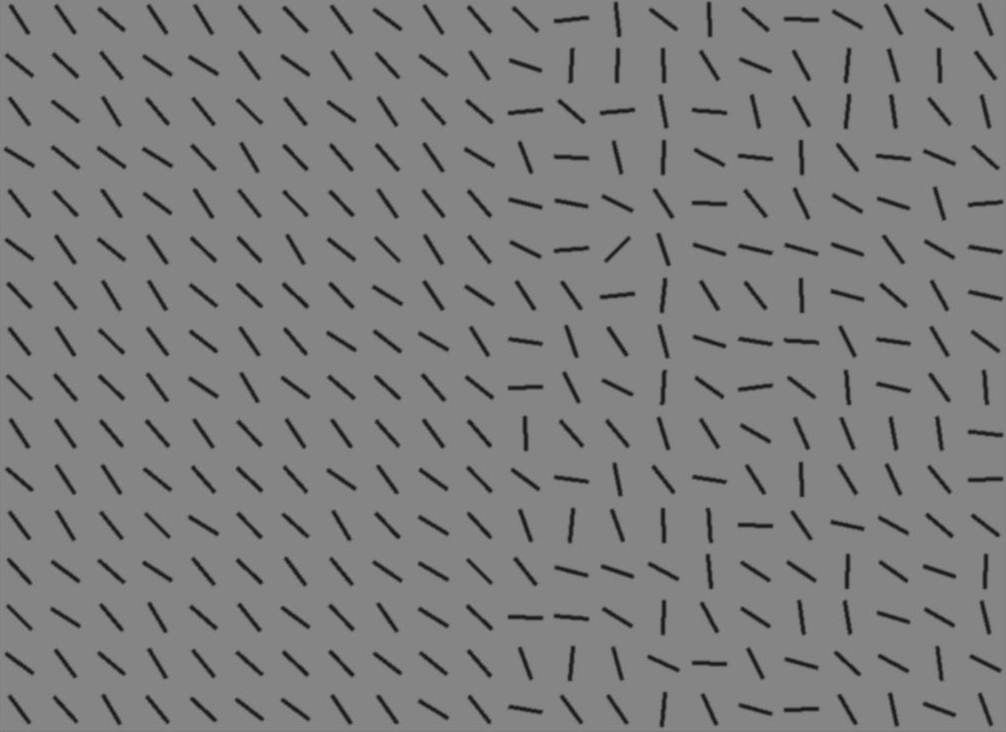
\includegraphics[height=3cm]{figures/split-half.png}}
\subfigure[][]{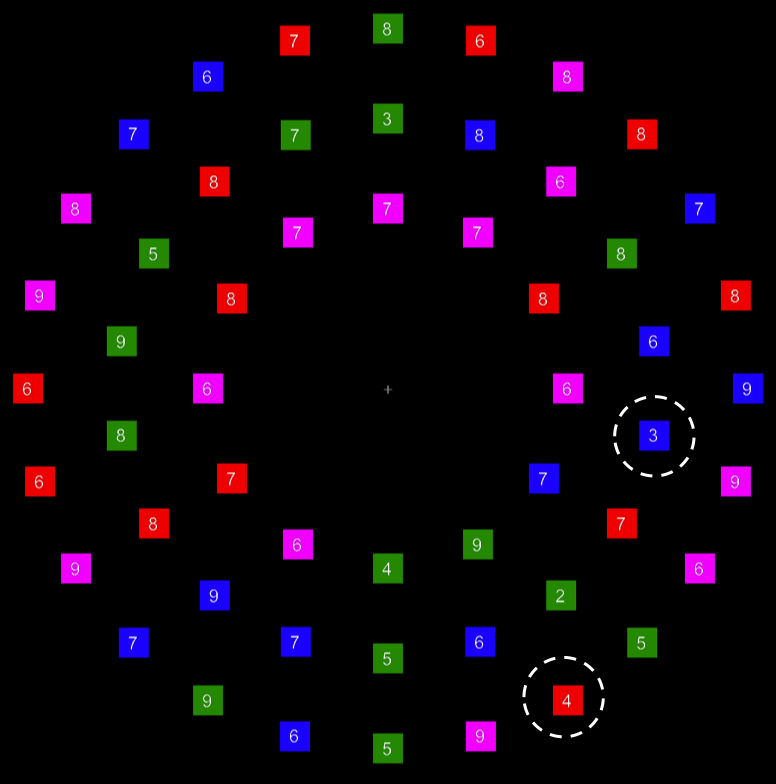
\includegraphics[height=3cm]{figures/adaptive.png}}
\subfigure[][]{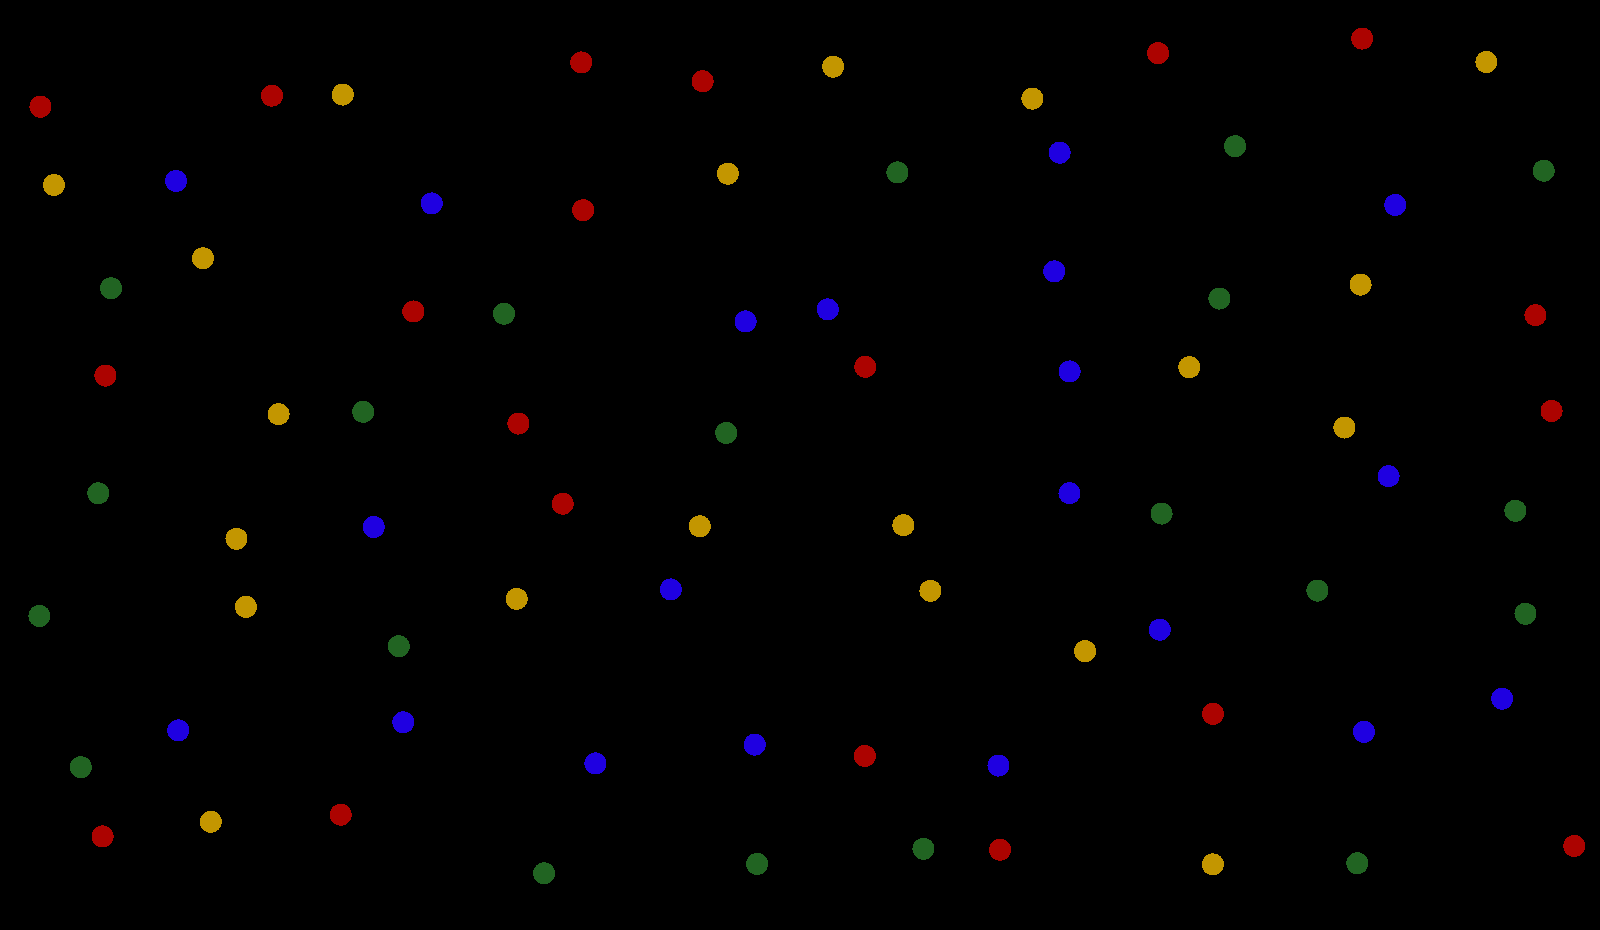
\includegraphics[height=3cm]{figures/foraging.png}}
\caption{Example stimulus from the (a) \textit{split-half}, (b) \textit{adaptive choice} and (c) \textit{foraging} paradigms}
\label{fig:exampleStimuli}
\end{figure}

The display was presented on a 17-inch CRT monitor with a resolution of $1024 \times 
768$. Stimulus generation, presentation and data collection were controlled by MATLAB and psychophysics toolbox \cite{brainard1997} run on a Powermac. 

\subsubsection{Split-half Array Search}

Stimuli consisted of arrays of black oriented line segments against a grey background. The target was oriented $45^{\circ}$ clockwise, while the distractor items had a random orientation with a mean of $45^{\circ}$ anti-clockwise. The variance was low ($18^{\circ}$) on one half of the display to create a homogeneous texture, and high ($95^{\circ}$) on the other side to create a heterogeneous texture. This means that when the target is present on the homogeneous side of the stimulus, it can be easily be detected with peripheral vision, but when it is in the heterogeneous half, it is much harder to detect. There were a total of 160 trials and homo- and heterogeneous sides of the display were randomly varied from trial to trial.
 
The position of the dominant eye was recorded using a desktop-mounted EyeLink 1000 eye
tracker (SR Research, Canada) sampling eye position at 1000 Hz.
This paradigm was carried out twice to give us an estimate of how consistent participants are in their search strategy over time. The two sessions were identical.

\subsubsection{Adaptive Choice Visual Search}

The ACVS was based on the task described in \cite{irons-leber2016}, with a few changes [Or identical to the task described in Experiment 1 of Irons \& Leber, in press by then hopefully].

Each search display was composed of 54 small squares (size? What was viewing distance \& screen size?) arranged in three concentric rings around fixation, with 12, 18 and 24 items in the inner, middle and outer rings respectively. The inner ring was $XX^{\circ}$ and the outer ring was $XX^{\circ}$ from fixation. Of the 54 squares, 13 were red, 13 were blue, 14 were green and 14 were "variable". Variable distractors changes colours from trial-to-trial according to a cyclical pattern: the distractors would be red for 5 trials (called a "red plateau"), then across a period of 7 trials, they would change colour from almost red to magenta (at the fourth trial in the transition) to almost blue (see \cite{irons-leber2017}, for the specific colour values? Or supplemental?). The variable distractor would then be blue for 5 trials (blue plateau), and then transition back from almost blue through magenta to almost red. This 24-trial cycle would repeat throughout the entire experiment. 

A white digit appeared inside each square. Two targets - a red square and a blue square each with a digit between 2 and 5 - were embedded in every search display. The two target digits were always different, to enable us to distinguish the chosen target. The remaining red, blue and variable squares all contained digits between 6-9. Green squares could contain any digit between 2-9. The location of the targets and distractor within the search display were randomized on each trial.

Participants were informed that the search displays would contain two targets on every trial, that they need only find one target on each trial and that they were always free to search for either one. A trial began with a 1.5s ITI containing a central fixation cross, followed by the search display until a response was made. Participant responded by pressing a key that corresponded to the digit inside the target (\texttt{V}, \texttt{B}, \texttt{N} and \texttt{M} keys corresponding to 2, 3, 4 and 5 respectively). Participants completed 10 practice trials, followed by 3 blocks of 96 trials. Each block started on a red plateau.  

\subsubsection{Conjunction Foraging}

The foraging task was based on \cite{kristjansson2014} and \cite{johannesson2016}. Participants completed the feature foraging and conjunction foraging tasks on separate days, with the order counterbalanced (was it counterbalanced?).

In the feature foraging task, search displays contained 80 small circles (size), 20 red (RGB: 180, 0, 0), 20 green (RGB: 20, 100, 40), 20 blue (RGB: 0, 0, 220) and 20 yellow (RGB: 200, 150, 0), presented against a black background. Stimuli were arranged in a 10 x 8 grid, but the position of each item within the grid space was jittered to create a more random spatial arrangement (with the restriction that two items could not be within 30 pixels of each other). The location of item colours to grid locations was completely randomized. 
For half of the participants, targets were red and green circles, and for the other half of participants, targets were blue and yellow circles. Participants were asked to collect all of the targets within a trial by using the mouse to click on each target. Clicking on a target caused it to disappear from the display. If the participant clicked erroneously on a non-target, the trial was immediately ended and a replacement trial was begun. Participants completed 1 practice trial and 20 full-completed experimental trials.

In the conjunction foraging task, search displays were composed of both circles and squares. For half of the participants, the shapes were red and green (equal numbers of red circles, red squares, green circles and green squares), and for the remaining participants the shapes were blue and yellow. Targets were defined by conjunctions of colour and shape (e.g., red squares and green circles, with red circles and green squares as distractors). The assignment of targets and distractors was assigned at random for each participant. The procedure was otherwise identical to the feature foraging task. 

%% For the assignment of distractors and targets, we generated a two lists of random numbers (1-2 for easy search, and 1-4 for hard search). Pretty sure we did that because counterbalancing became very tricky once you accounted for that as well. 
\subsection{Planned Analysis}

\subsubsection{Split-half array search}

In order to characterise an individual's behaviour in this task, we will compute the proportion of the first $n$ fixations that were on heterogeneous (difficult) side of the stimuli, over all target absent trials\footnote{Only take correct trials?}. \cite{nowakowsak2017} demonstrated a strong correlation between an this metric (for $n=5$) and reaction times ($r=.53$). However, a re-analysis of their data shows that an even stronger correlation is obtained with $n=3$.

\subsubsection{Attentional Control}

Participants with accuracy more than 3 SD below the group mean were excluded from analyses. For RT analyses, trials with RTs less than 300ms or more than 3 SD about the participant's mean were excluded. 

Two measures of individual strategy use were used: 1) Optimal choices, defined as percent of plateau trials in which the individual chose the optimal target (i.e., the target with the fewest distractors. When the variable distractor was red, the optimal choice was blue, and vice versa), and 2) Switch rate, the percent of trials in which the individual switched target colour (i.e., the colour chosen on trial N was different to the colour chosen on trial N-1).  

\subsubsection{Conjunction Foraging}

Only completed, accurate trials were analysed. RTs were defined across the entire trial (i.e., from the start of the trial until the final target was collected). The main measure of interest was average run length per trial. A run was defined as a succession of one or more of the same target type, which was followed and preceded by the other target or no target. The average run length was the average number of target selections in a run. 

\subsection{Exploratory Analysis}

We will carry out additional analysis, above and beyond what has been documented above, but the exact nature of this will be contingent on the nature of the results. Something like PCA may be interesting. 

%%%%%%%%%%%%%%%%%%%%%%%%%%%%
\section{Results}
%%%%%%%%%%%%%%%%%%%%%%%%%%%%

\subsection{Replication of each paradigm}

\subsubsection{Split-half Array Search}
Our results are broadly in line with \cite{nowakowsak2017}. The correlation between accuracy and reaction times between the two sessions is shown in Figure \ref{fig:splithalf_summary}(a, b). We can clearly see that there are large differences from one participant to the next in terms of both the proportion of hard targets found, and reaction times. Furthermore, test-retest reliability appears to be reasonable, with correlations of around $r = 0.78$ (the value of $r = 0.71$ or easy targets is slightly lower, likely due to the restricted range).

\begin{figure}
\centering
\subfigure[][]{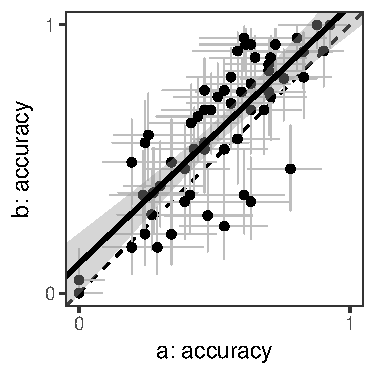
\includegraphics[width=5cm]{../Scripts/lineseg/scratch/acc_correlation.pdf}}
\subfigure[][]{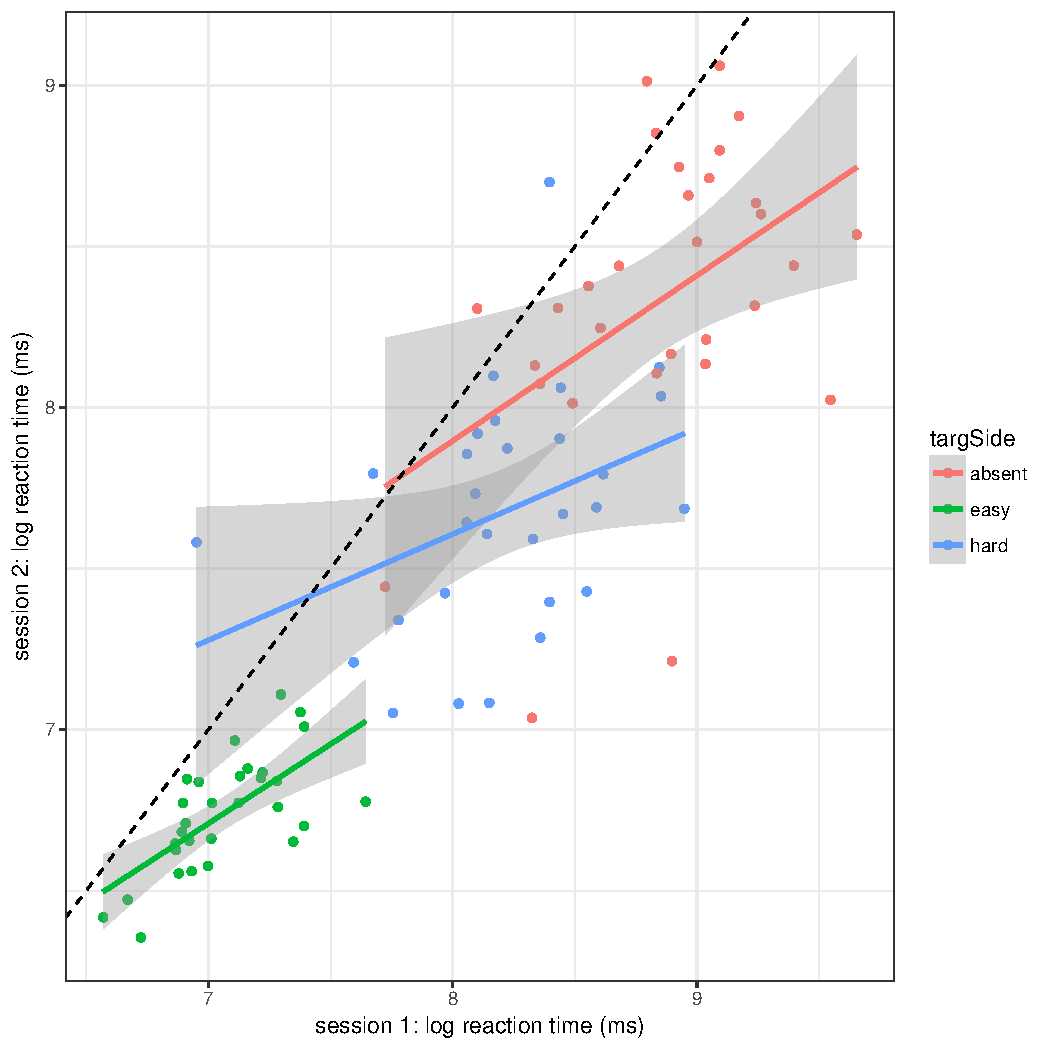
\includegraphics[width=5cm]{../Scripts/lineseg/scratch/rt_correlation.pdf}}
\subfigure[][]{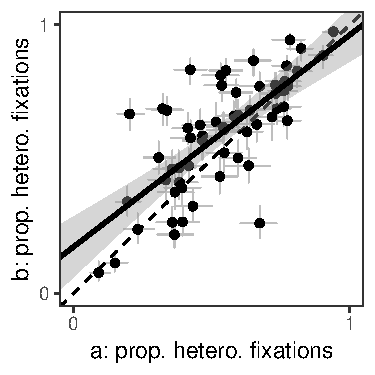
\includegraphics[width=5cm]{../Scripts/lineseg/scratch/strat_corr.pdf}}
\subfigure[][]{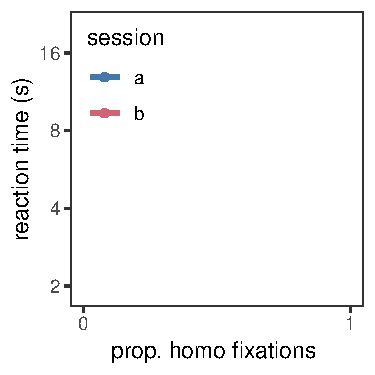
\includegraphics[width=5cm]{../Scripts/lineseg/scratch/strat_compare_meanlog_rt.pdf}}
\caption{Correlation between the two sessions of the \textit{split-half} paradigm for (a)  accuracy (TP-heterogeneous), (b) reaction times and (c) search strategy. (d) initial search strategy correlates with reaction times in both sessions. Each point represents a participant and the error-bars indicate 95\% confidence intervals.}
\label{fig:splithalf_summary}
\end{figure}

We can also look at the initial search strategies adopted by our participants \ref{fig:splithalf_summary}(c, d). Again, we see large and stable individual differences across the two sessions. More importantly, as with \cite{nowakowsak2017}, we see that the search strategies give a good correlation with reaction times. 


\subsubsection{Adaptive Choice}

\subsubsection{Conjunction Foraging}


\subsection{Correlations Between Paradigms}

The results above demonstrate that we have successfully replicated the previous findings around individual differences in visual search strategy. We now investigate whether there are correlations between paradigms: are individuals who are good at one visual search task good at another? We start by looking at simple reaction times (Figure \ref{fig:between_para_rt}). In all comparisons the correlations are weak, typically $0.27 < r <0.30$ but positive. None of these correlations are statistically significant ($p>0.05$). Even if we optimistically take all the data together as suggesting a robust correlation in reaction times from paradigm to paradigm, the upper bound of $r=0.30$ this correlation only accounts for at best $10\%$\footnote{i.e., $R^2 = 0.3^2 = 0.09$} an individual's performance. 


\begin{figure}
\centering
\subfigure[][]{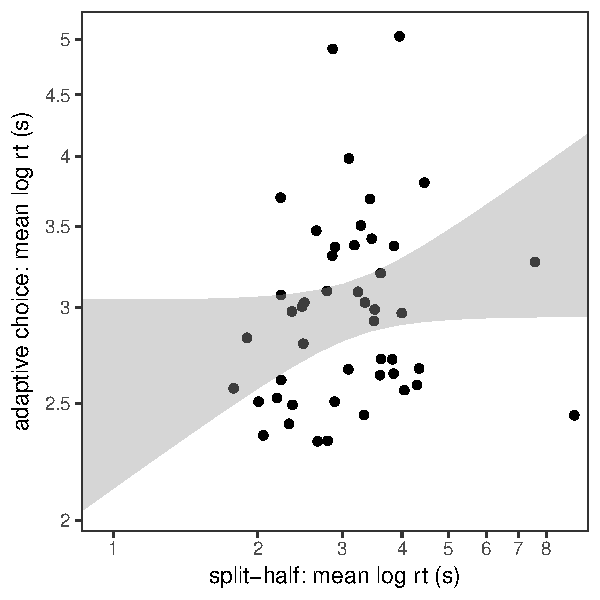
\includegraphics[width=5cm]{../Scripts/scratch/ls_v_ac_mean_log2rt.pdf}}
\subfigure[][]{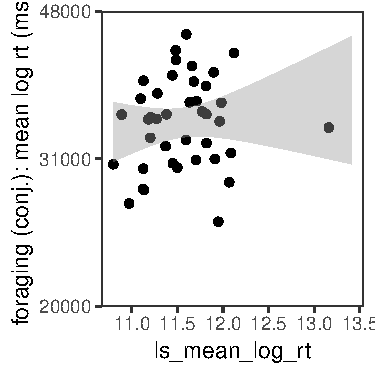
\includegraphics[width=5cm]{../Scripts/scratch/ls_v_fg_conj_rt.pdf}}
\subfigure[][]{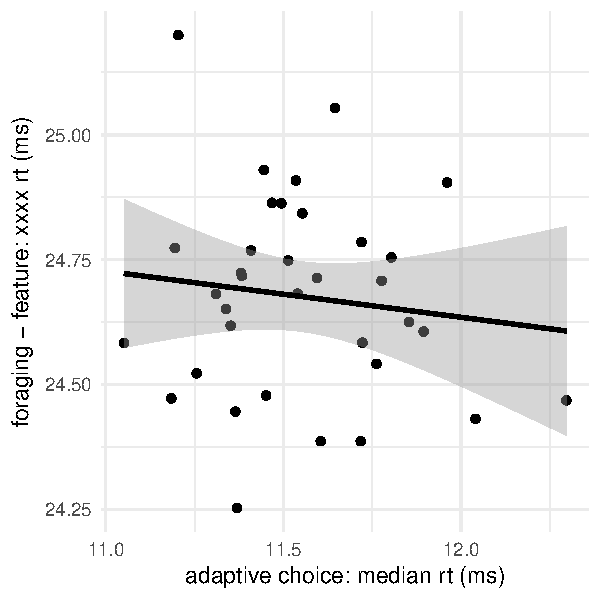
\includegraphics[width=5cm]{../Scripts/scratch/ac_v_fg_feature_rt.pdf}}
\subfigure[][]{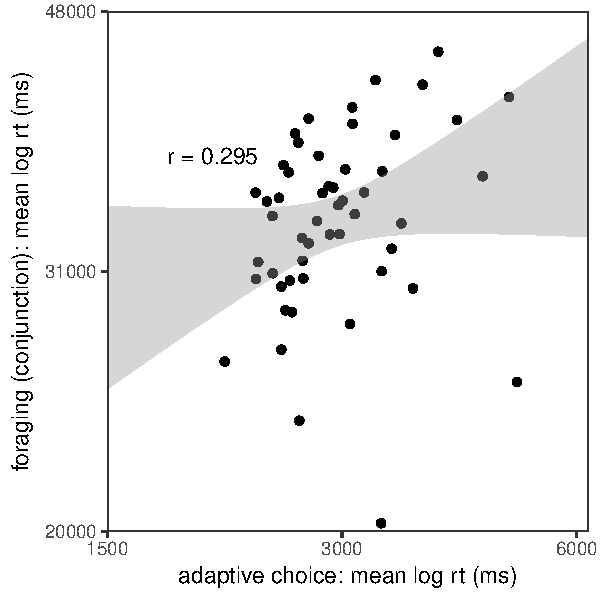
\includegraphics[width=5cm]{../Scripts/scratch/ac_v_fg_conj_rt.pdf}}
\subfigure[][]{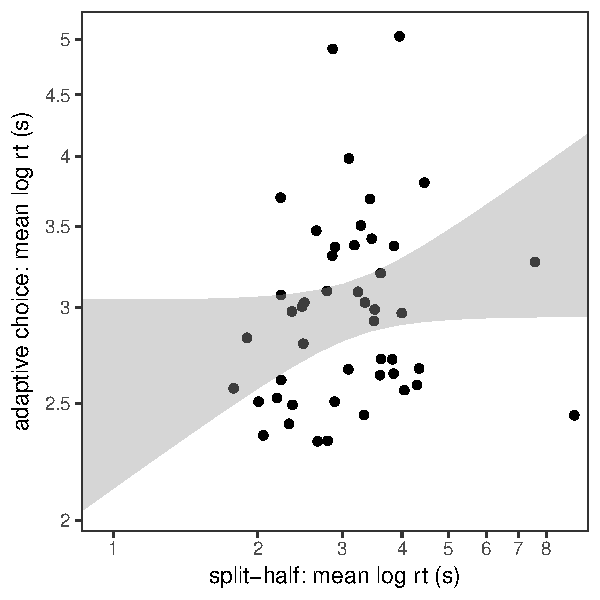
\includegraphics[width=5cm]{../Scripts/scratch/ls_v_ac_mean_log2rt.pdf}}
\caption{Correlation a) split-half and feature foraging; b) split-half and conjunction foraging, c) adaptive choice and feature  foraging; d) adaptive choice and conjunction foraging; e) split-half and adaptive choice. In all cases, these correlations are low, with $p>0.05$}
\label{fig:between_para_rt}
\end{figure}

Given the low correlations between reaction times, it seems unlikely that we will find that individuals who search efficiently and optimally in one paradigm will search well in another (the original motivation for our study). The analysis supports this hypothesis. For example, the correlation between the proportion of fixations to the heterogeneous side of the display in the split-half paradigm, and proportion of optimal targets found in the adaptive choice task is $r=-0.03$. Further results are presented in supplementary materials. 

%%%%%%%%%%%%%%%%%%%%%%%%%%%%
\section{Discussion}
%%%%%%%%%%%%%%%%%%%%%%%%%%%%

The results presented above are somewhat surprising. 

\bibliographystyle{plain}
\bibliography{literature}

\end{document}


